\documentclass[3pt,twocolumn]{elsarticle}
\usepackage[spanish]{babel}
\usepackage[utf8]{inputenc}
\usepackage[T1]{fontenc}
\usepackage{lineno,hyperref}
\modulolinenumbers[5]
\usepackage{graphicx}
\usepackage{subcaption}
\usepackage{listings}
\lstset{language=R, breaklines=true}
\usepackage{url} % UTILIZA EL PAQUETE PARA QUE APAREZCA EL URL AUNQUE AUN NOSE SI DEBO ACTIVARLO TAMBIEN EN REFERENCIAS
\hypersetup{
    colorlinks=true,
    linkcolor=blue,
    filecolor=blue,      
    urlcolor=blue,
}
\usepackage{amsmath}
\bibliographystyle{elsarticle-num}
\captionsetup[subfigure]{labelformat=brace}

\makeatletter

\renewenvironment{abstract}{\global\setbox\absbox=\vbox\bgroup
  \hsize=\textwidth\def\baselinestretch{1}%
  \noindent\unskip\textbf{Resumen}  % <--- Edit as necessary
 \par\medskip\noindent\unskip\ignorespaces}
 {\egroup}

\def\keyword{%
  \def\sep{\unskip, }%
 \def\MSC{\@ifnextchar[{\@MSC}{\@MSC[2000]}}
  \def\@MSC[##1]{\par\leavevmode\hbox {\it ##1~MSC:\space}}%
  \def\PACS{\par\leavevmode\hbox {\it PACS:\space}}%
  \def\JEL{\par\leavevmode\hbox {\it JEL:\space}}%
  \global\setbox\keybox=\vbox\bgroup\hsize=\textwidth
  \normalsize\normalfont\def\baselinestretch{1}
  \parskip\z@
  \noindent\textit{Palabras clave: }  % <--- Edit as necessary
  \raggedright                         % Keywords are not justified.
  \ignorespaces}

\def\ps@pprintTitle{%
     \let\@oddhead\@empty
     \let\@evenhead\@empty
     \def\@oddfoot{\footnotesize\itshape
        \ifx\@journal\@empty Simulación computacional de nanomateriales  % <--- Edit as necessary
       \else\@journal\fi\hfill\today}%
     \let\@evenfoot\@oddfoot}

\makeatother

\begin{document}

\twocolumn[
\begin{@twocolumnfalse}
\begin{frontmatter}
\title{Modelado del fenómeno de maduración de Ostwald}
\author{Garcia Fuentes J. A. \\ Correo electrónico: \href{mailto:jose.garciafnt@uanl.edu.mx}{jose.garciafnt@uanl.edu.mx}}
\address{Facultad de Ingeniería Mecánica y Eléctrica, Universidad Autónoma de Nuevo León}


\begin{abstract}
Se muestra un descripción de los sistemas que tienden a descomponerse mediante una variedad de mecanismos fisicoquímicos enfocando principalmente al fenómeno de maduración de Ostwald, se presenta un modelo del fenómeno tomando en cuenta el Movimiento Browniano que tienen las partículas, así como también una carga electrostática y una masa que influyen en el tamaño de estas de acuerdo al fenómeno.
\end{abstract}

\begin{keyword}
Floculación \sep Emulsión \sep Carga \sep Browniano \sep Simulación
\end{keyword}
\end{frontmatter}
\end{@twocolumnfalse}
]

\section{Introducción}


Las emulsiones son sistemas termodinámicamente desfavorables que tienden a descomponerse con el tiempo debido a una variedad de mecanismos fisicoquímicos (Figura \ref{ostwlad}), incluida la separación gravitacional, la floculación, la coalescencia y la maduración de Ostwald \cite{a1}. El engrosamiento de la textura (también conocido como maduración de Ostwald, equilibrio o maduración de la textura) se ha propuesto como un proceso importante en rocas plutónicas y algunas rocas volcánicas. En un contexto ígneo, el engrosamiento es la reabsorción de cristales pequeños y el crecimiento simultáneo de cristales más grandes como un proceso de minimización de la energía superficial total (libre). Aunque no existe consenso sobre el proceso exacto de engrosamiento de la textura, se utiliza la teoría de Comunicando Vecinos y la teoría Lifshitz-Slyozov-Wagner \cite{a9}. Durante la maduración de Ostwald , se consumen cristales dispersos por debajo de un radio crítico, mientras que los granos mayores continúan creciendo a expensas de los más pequeños el radio critico no es una constante, sino que aumenta con el tiempo. Esto se debe a que el sistema no estará en un equilibrio termodinámico estable hasta que todo el material de un determinado mineral se reúna en un solo cristal, o al menos hasta que todos los granos en un determinado dominio rocoso tengan aproximadamente el mismo tamaño \cite{a2}.

Una vez que cesó la nucleación y/o el crecimiento del sistema abierto, quizás debido al agotamiento de un determinado elemento en el reservorio, no se formarán nuevos cristales y las poblaciones existentes pueden continuar creciendo de manera que minimizan su energía libre superficial \cite{a2}.
En la mayoría de las muestras, la evolución temporal alcanza rápidamente un estado estable. Sin embargo algunas muestras como plagioclasa en fundidos de silicato, el tamaño de los cristales se amortigua rápidamente, ya que en los fundidos de silicato se ha interpretado principalmente como una maduración controlada por un proceso de nucleación superficial en la interfaz cristal-líquido \cite{a3}.
Para algunos modelos se pueden mencionar 3 etapas basicas en la maduracion empezando por una evolución microestructural durante la transformación de fase. La nucleación heterogénea inicial a partir del grano en descomposición da como resultado un intercrecimiento a lo largo de los límites del grano. En la naturaleza, este intercrecimiento se conoce como kelifita o simplicidad de grano. Sin embargo, en algunos casos las escalas de tiempo de engrosamiento son largas, lo que resulta en un engrosamiento del borde de reacción. Si el sistema evoluciona lo suficientemente lento como para que la microestructura avance más hacia el equilibrio, el intercrecimiento se concentrará alrededor de uniones triples. Finalmente, si el sistema avanza más hacia el equilibrio, los pequeños granos intersticiales serán absorbidos por vecinos más grandes
\cite{a5}.
	\begin{figure}[h!]
				\centering
				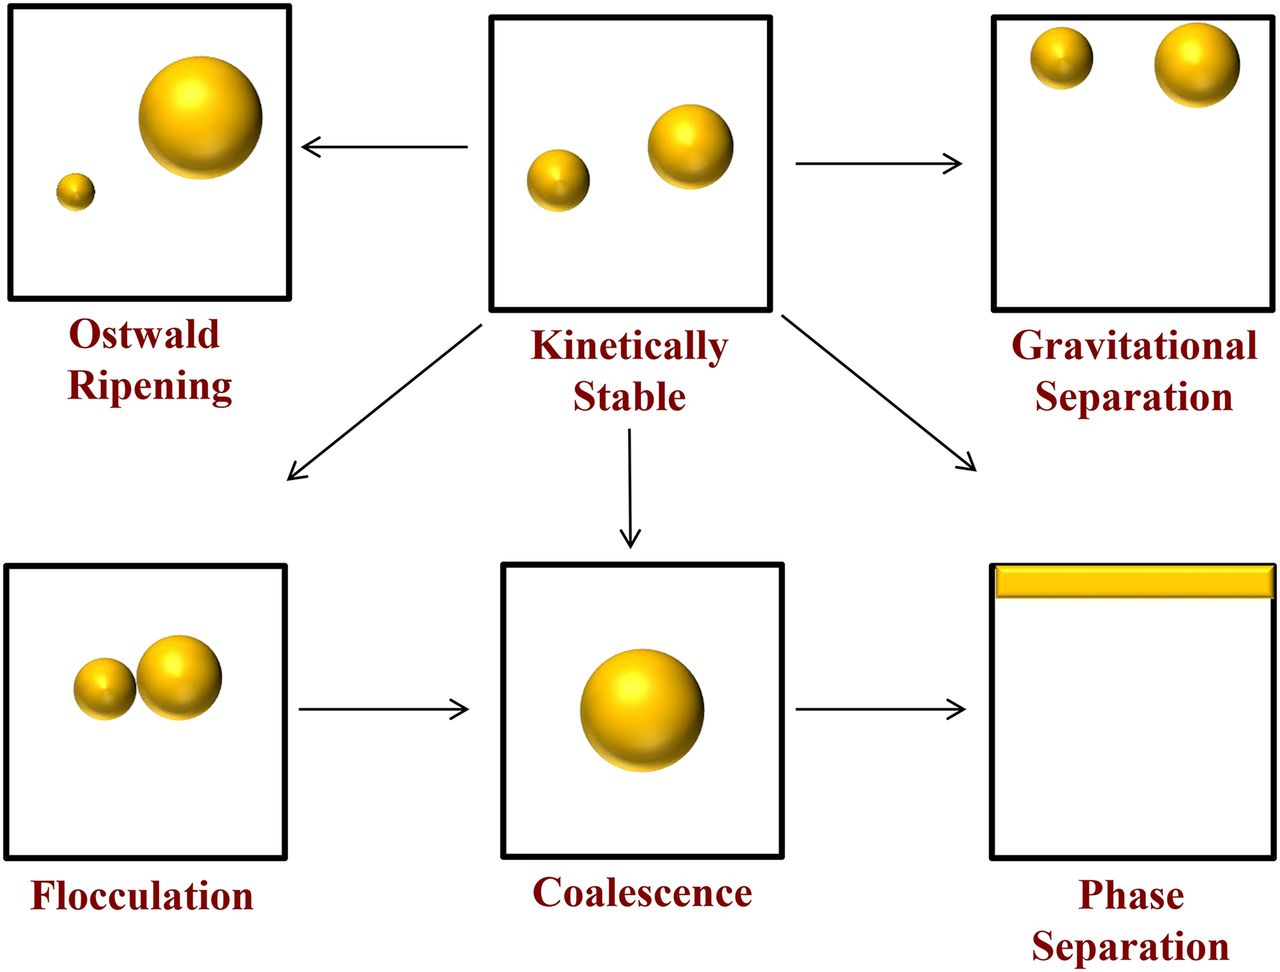
\includegraphics[scale=0.7]{ostwlad.jpeg} 
				\caption{Diagrama esquemático de los mecanismos de inestabilidad más comunes que ocurren en los sistemas de administración coloidal: separación gravitacional, floculación, coalescencia, maduración de Ostwald e inversión de fase \cite{a1}.}
		\label{ostwlad}
\end{figure}

La superposición rítmica de escala fina es otra variedad de superposición difusa de este tipo. Normalmente se encuentra en una escala de unos pocos centímetros y se cree que se debe a un proceso de reequilibrio en el que pequeñas diferencias iniciales de tamaño de grano o proporciones modales se acentúan y repiten por la solución cíclica y el crecimiento de cristales en condiciones similares a las de Maduración de Ostwald
\cite{a6}.

En el presente trabajo se planea realizar una simulación con modelado del fenómeno de maduración de Ostwald empleando los modelos de Movimiento Browniano, y adecuando a cada partícula una carga y una masa, el modelado se describe en mayor detalle en la sección de resultados y discusión.


\section{Maduración de Ostwald}
La maduración de Ostwald se debe al crecimiento de las gotas más grandes a costa de las más pequeñas, hasta que estas últimas prácticamente desaparecen. El proceso va de acuerdo con una velocidad que está en función de la solubilidad de la fase, dispersa en la fase continua y se debe a que la presión interna de las gotas, la presión es mayor a las gotas más pequeñas \cite{a15}. La maduración de Ostwald estará ocurriendo tan pronto como las interfaces curvas están presentes, ya que esta curvatura causa alta solubilidad desde la fase dispersa en el límite de la partícula comparada con la fase volumétrica proxima. A las partículas grandes el gradiente de concentración de la fase, dispersa en la fase continua, provoca partículas grandes que crecen a expensas de las más pequeñas ( figura \ref{a14i}) \cite{a14}.
La maduracion se dirige por la diferencia de la presión entre gotas que tiene diferentes radio, por lo que la fase dispersa se difunde de las gotas más pequeñas a las de mayor tamaño, la transferencia de masa en emulsiones no sólo se dirige por la diferencia en la curvatura de las gotas, sino también por la diferencia de sus composiciones \cite{a15}. Algunos autores mencionan los efectos muy menores en los cristales de más de $20 \mu m$. De acuerdo con esto, estas porciones más gruesas del umbral no se distinguen por densidades de población especialmente altas en las clases de tamaño de cristal más grande. Más bien, tienen densidades de población especialmente bajas en las clases de tamaño de cristal pequeño \cite{a7}.


	\begin{figure}[h!]
				\centering
				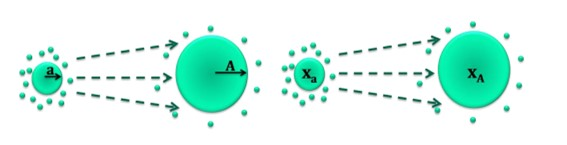
\includegraphics[scale=0.5]{a14.jpg} 
				\caption{Trasferencia de masa en emulsiones mixtas \cite{a14}}
		\label{a14i}
\end{figure}

Este proceso espontáneo, controlado termodinámicamente \cite{a4}, se produce porque las partículas más grandes están energéticamente favorecidos con respecto a las más pequeñas. Esto proviene del hecho de que las moléculas en la superficie de una partícula son energéticamente menos estables que los que están en el interior. Cuando todas las partículas pequeñas hacen esto, aumenta la concentración de moléculas libres en solución. Cuando las moléculas libres en solución se sobresatura, las moléculas libres tienen una tendencia a condensarse sobre la superficie de las partículas más grandes. Por lo tanto, las partículas más pequeñas se reducen, mientras que las partículas grandes crecen, y en general el tamaño medio irá en aumento. Como un tiempo infinito, la población entera de partículas se convierte en una partícula esférica grande para minimizar la superficie total.

\subsection{Agregación y engrosamiento}
Tanto la agregación como el engrosamiento son procesos estrechamente relacionados de importancia en la formación de acumulados. La agregación es un término general que describe la agrupación de granos en una masa fundida. En algunos casos, los cristales parecen estar adheridos a lo largo de caras cristalográficamente similares, lo que garantiza que se minimice el desajuste estructural y la energía interfacial. Por el contrario, también se ha propuesto que el crecimiento se ve reforzado por la anexión de granos pequeños por cristales más grandes, seguida de la migración de los límites de los granos \cite{a9}.

\subsection{Disolución-reprecipitación en la masa de cristales}
Con subenfriamientos bajos, la distribución del tamaño de grano de una suspensión polidispersa dentro de un líquido evoluciona bajo la influencia de energías interfaciales. La mayor energía libre de los cristales pequeños en relación con los cristales más grandes significa que los granos grandes crecen a expensas de los más pequeños. El efecto del tamaño sobre la solubilidad equivale a un sobrecalentamiento efectivo de los cristales más pequeños. Este proceso tiene un efecto insignificante si los cristales están muy separados, particularmente para granos de más de unas pocas micras, pero ocurre a una velocidad mayor cuando los cristales se tocan, ya que los granos pueden coalescer o si hay ciclos térmicos. La pérdida de granos pequeños también puede ocurrir por disolución preferencial causada por el estrés resultante de la presión del material superpuesto en la pila de cristales \cite{a10}. 




\section{Experimentación}
Se toman en cuenta distintos puntos los cuales se asocian de diferentes maneras como el número de cristales, el tamaño de los cristales y el tiempo de cristalización. Esto introduce tres constantes características que solo se pueden encontrar empleando modelos cinéticos específicos de cristalización. El tiempo característico de cristalización depende solo débilmente de la cinética exacta de cristalización, pero el número y tamaño de cristal típicos son más sensibles a la cinética; la nucleación y el crecimiento pueden estar relacionados exponencialmente con el tiempo, el tamaño de los cristales es principalmente el resultado de la nucleación heterogénea y la anexión de grano rápida y continua y la migración de los límites \cite{a8}. Otra característica a tomar en cuenta es el estudio del potencial de la partícula (carga electrostática) ya que a un mayor potencial electrostático se proporciona una mayor estabilización \cite{a11,a12} Los cambios en la tasa de crecimiento y nucleación fuera de las condiciones constantes alterarán la pendiente y la intersección una población de cristales (Temperatura) \cite{a13}. 

\subsection{Herramientas}
La simulación se realizó en una laptop-dfbogt8t con un procesador AMD Ryzen 5. Para la simulación se utilizó el paquete estadístico R  \cite{R} para generar visualizaciones y analisis de resultados.

\subsection{Simulación}
La simulación se llevó a cabo en base a los códigos relacionados al comportamiento browniano \cite{p1} e interacciones entre partículas \cite{p7} con la finalidad de agregar un movimiento aleatorio de una partícula en una solución y ver como interactúan los factores como la masa, la energía electrostática y la temperatura al generar partículas de mayor tamaño simulando el fenómeno de Ostwald.

\subsection{Análisis de resultados}
Se calcula el número de partículas iniciales de la simulación comparando con el número de partículas finales el cual se requiere que sea una sola, se requiere obtener el tiempo que pasa desde el inicio al final del fenómeno, el tiempo es otro factor a tomar en cuenta al modificar la temperatura para retardar o acelerar el fenómeno.

\section{Resultados y discusión}

\section{Conclusiones}

Se requeriría realizar la simulación nuevamente en el futuro, incluyendo propiedades específicas de un material y una solución con la finalidad de obtener datos informativos sobre la saturación o sobresaturación de una solución o bien para aprovechar las energías libres de los compuestos ya sea para estabilizar un fluido o emulsión o bien mantenerlo siempre activo con la adicción de algún otro compuesto.
Se deberá tomar en cuenta que la aglomeración tipo Ostwald también depende de fenómenos como floculación o agregación que de cierta manera aceleraran el proceso debido a que estas partículas siempre están en movimiento lo que provocaría una coalescencia.

\subsection{Trabajos futuros}

\section{Agradecimientos}
Se agradece encarecidamente a la Dra. Elisa Schaeffer por sus correcciones en la estructura original del trabajo y las bases enseñadas para el desarollo de el mismo.

\bibliography{referencias}

\end{document}
